\documentclass[11pt]{article}

\usepackage{ppackage}
\usepackage{bbm}
\usepackage{import}






\usepackage{tikz}
\usetikzlibrary{arrows.meta,patterns}
\usetikzlibrary{ipe} % ipe compatibility library

\usepackage{../../Notes/tikzit}
\usepackage{../../Notes/utf8math}

\input{../../Notes/TIKZ/digraph.tikzstyles}



\usepackage{url}


\newcommand{\solution}{
\bigskip\noindent
	\textbf{Solution: \\}}
	


\DeclareMathOperator{\size}{size}
\DeclareMathOperator{\conv}{conv}
\newcommand{\SV}{\mathrm{SV}}
\newcommand{\bigO}{O}
\newcommand{\cut}{\mathrm{cut}}
\newcommand{\LLL}{\mathrm{LLL}}
\newcommand{\setR}{\mathbb{R}}
\newcommand{\setZ}{\mathbb{Z}}
\newcommand{\setQ}{\mathbb{Q}}
\newcommand{\setC}{\mathbb{C}}
\newcommand{\setN}{\mathbb{N}}
\newcommand{\wt}[1]{\widetilde{#1}}
\newcommand{\opt}{{\sc 0/1-opt}\xspace}
\newcommand{\aug}{{\sc 0/1-aug}\xspace}
\newcommand{\psep}{{\sc 0/1-psep}\xspace}
\newcommand{\sep}{{\sc 0/1-sep}\xspace}
\newcommand{\fopt}{{\sc 0/1-testopt\xspace} }

\newcommand{\hpp}{\mathrm{HPP}}
\newcommand{\nodes}{\mathcal{V}}
\newcommand{\vol}{\mathrm{vol}}
\newcommand{\diag}{\mathrm{diag}}
\newcommand{\arcs}{\mathcal{A}}
\newcommand{\edges}{\mathcal{E}}
\newcommand{\paths}{\mathscr{P}}
\newcommand{\cycles}{\mathcal{C}}




\newcommand{\K}{{\mathcal K}}
\newcommand{\A}{{A}}
\newcommand{\B}{{B}}
\newcommand{\T}{\mathscr{T}}
\newcommand{\eE}{\mathscr{E}}
\newcommand{\eS}{\mathscr{S}}
\newcommand{\eP}{\mathscr{P}}
\newcommand{\eM}{\mathscr{M}}



\newcommand{\transp}{^{\mathrm{T}}}

\newcommand{\smallmat}[1]{\left( \begin{smallmatrix} #1 \end{smallmatrix}\right)}

\newcommand{\mat}[1]{ \begin{pmatrix} #1 \end{pmatrix}}
\newcommand{\smat}[1]{ \big(\begin{smallmatrix} #1 \end{smallmatrix}\big)}

\newcommand{\pc}{\mathscr{P}}
\newcommand{\ob}{\mathscr{O}}
\newcommand{\odds}{\mathscr{W}}
\newcommand{\up}{\mathscr{U}}
\newcommand{\ef}{\mathscr{F}}
\newcommand{\eh}{\mathscr{H}}
\newcommand{\ev}{\mathscr{V}}
\newcommand{\ec}{\mathscr{C}}
\newcommand{\eu}{\mathscr{U}}

\newcommand{\lex}{\mathrm{lex}}

\renewcommand{\leq}{\leqslant}
\renewcommand{\geq}{\geqslant}









\newcommand{\linhull}{\mathrm{lin.hull}}
\newcommand{\affhull}{\mathrm{affine.hull}}
\newcommand{\charcone}{\mathrm{char.cone}}
\newcommand{\cone}{\mathrm{cone}}
\newcommand{\rank}{\mathrm{rank}}
\newcommand{\wb}[1]{\overline{#1}}



\usepackage{enumerate}

      
\institute{\'Ecole Polytechnique F\'ed\'erale de Lausanne}
\lecture{Discrete Optimization}
\faculty{Prof. Eisenbrand}
\term{Spring 2025}
\publishdate{May 6, 2025}
\duedate{ }
\problemset{Assignment~11}

\begin{document}
\makeheader

\begin{enumerate}[1)]
\item Find a maximum cardinality matching and a minimum cardinality vertex cover in the following graph.
  \begin{center}
    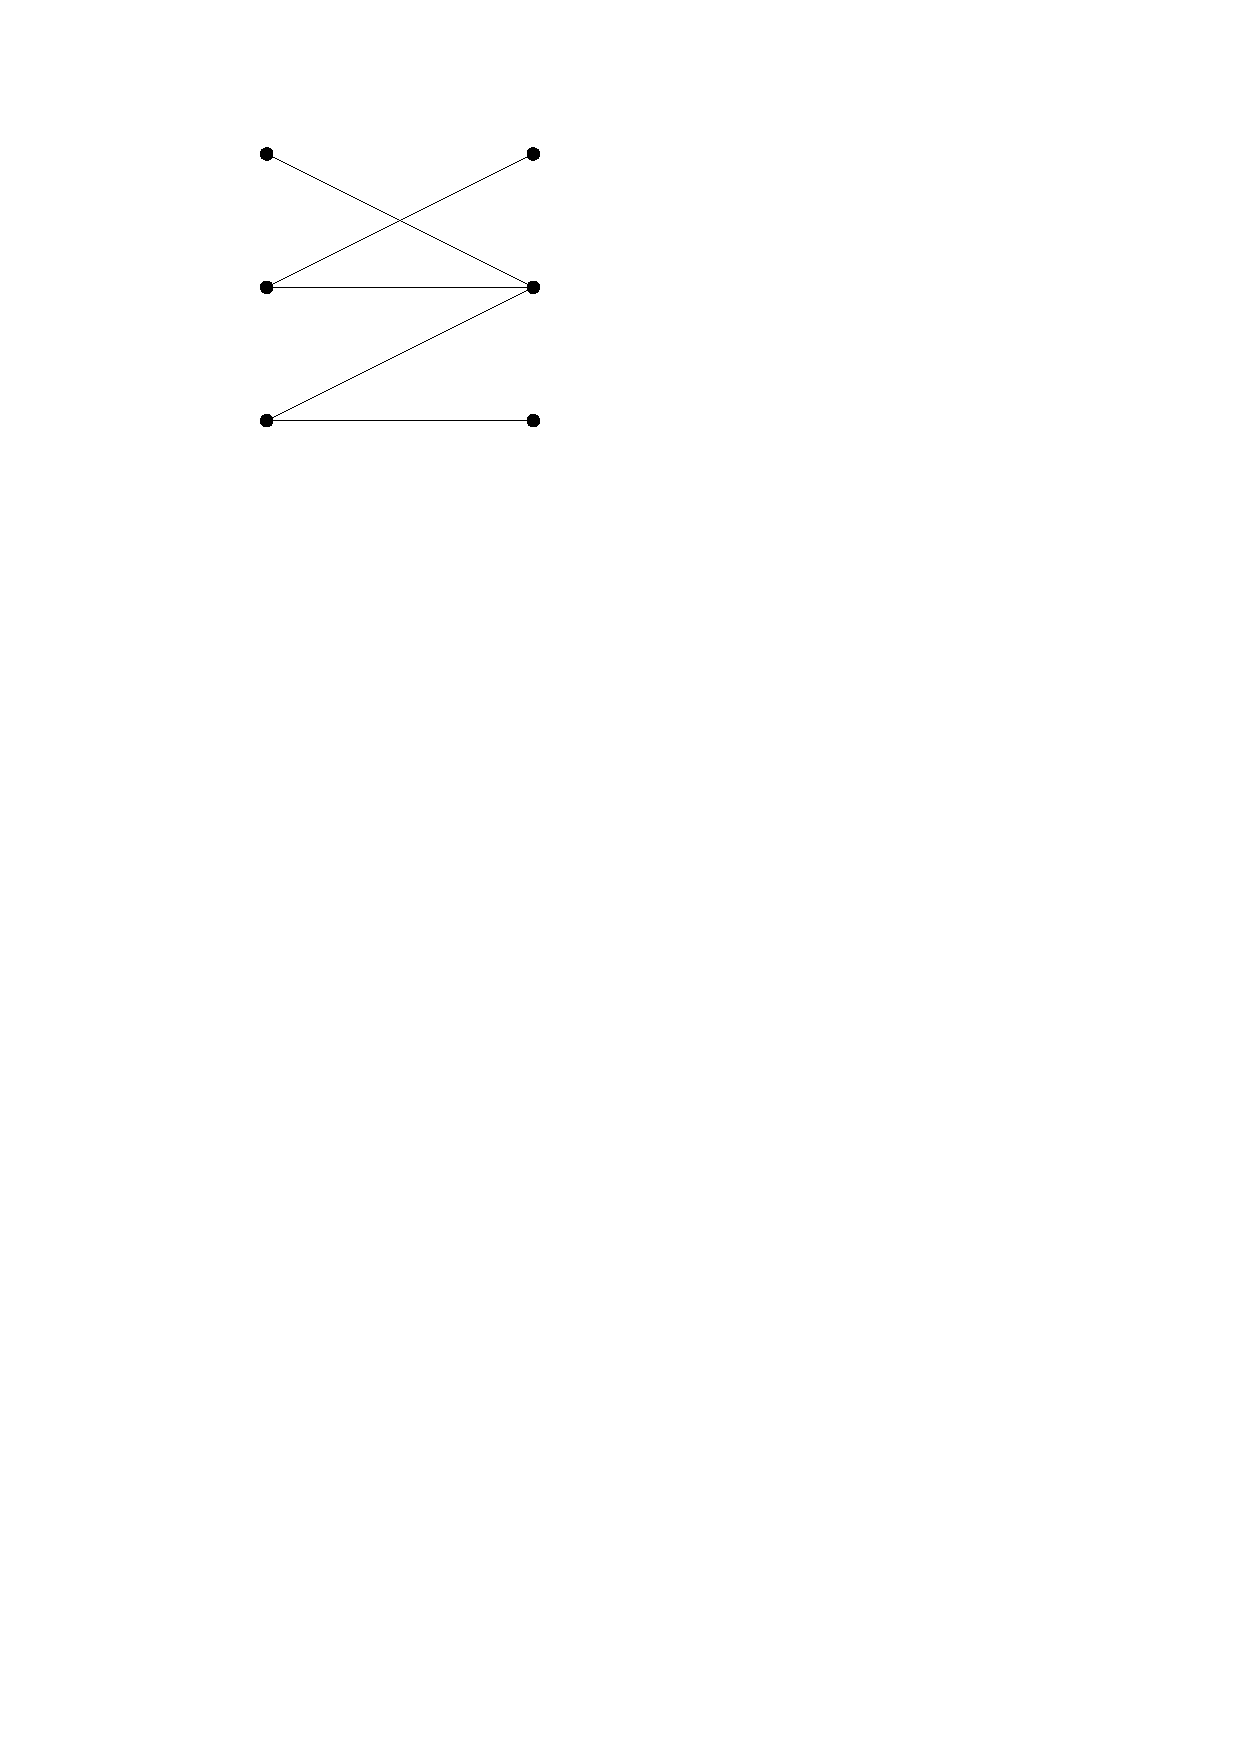
\includegraphics[width=0.2\textwidth]{graph1}
  \end{center}
\item Let $D = (V,A)$  be a directed graph and $A_D ∈ \{0,\pm1\}^{|V| × |A|}$ be the node-edge incidence matrix of $D$. Assume that the underlying undirected graph $G = (V,E)$  with $E = \{ uv : uv ∈A \text{ or } vu ∈ A\}$ is connected. 
  \begin{enumerate}[i)]
  \item Show that any row of $A_D$ is in the span of the other rows.
  \item Let $T ⊆ A$ be a selection of $n-1$ arcs of $A$ such that the induced undirected graph is a spanning tree of $G$. Show that the corresponding columns of $A_D$ are linearly independent.
  \end{enumerate}
  \item Consider the following problem. We are given $B\in \N$, and a set of integer points 
$$S=\{p\in \Z^n: \ 0\leq p_i\leq B, \ \forall i=1,\dots,n\},$$ 
whose points are all colored blue but one, which is red. We have an oracle that, given $i \in \{1,\dots,n\}$ and $\alpha \in \{0,\dots,B\}$, tells us whether there exists a red point $x^* \in S$ with $x^*_i \leq \alpha$. 
% given vectors $l, r\in \R^n$, tells us whether the red point in $S$ is contained in the box $S\cap\{x\in \R^n: l_i\leq x_i\leq r_i \;\forall\; i=1,\dots,n\}$ or not.

\medskip
\noindent 
Give an algorithm to find the red point using $O(n\log(B))$ many oracle calls.


\item 
  Let $Ax \leq b$ be a system of inequalities where each component of $A$ and $b$ is an integer bounded by $B$ in absolute value. Show that $Ax \leq b$ is feasible if and only if
  \begin{displaymath}
    \begin{array}{lc}
&      Ax \leq b \\
  i \in \{1,\dots,n\} : &      -(B n)^{n+1} \leq x_i \leq (Bn)^{n+1}  
    \end{array}
  \end{displaymath}
 \smallskip
 
Hint: Consider a feasible point $x^*$ and the index sets $I = \{i : \ x^*_i \geq 0\}$ and $J = \{j : x^*_j \leq 0\}$. The polyhedron defined by $Ax \leq b, \ x_i \geq 0, \ i \in I, \ x_j \leq 0, \ j \in J$ is feasible and has vertices. Estimate the infinity norm of a vertex with the Hadamard bound.  


\end{enumerate}




  

\end{document}

%%% Local Variables:
%%% mode: latex
%%% TeX-master: t
%%% End:
